\documentclass[a4paper]{../phyreport}

\usepackage{circuitikz}
\expName{电感的测量}
\expDate{2024}{3}{22}
\subDate{2024}{3}{29}
\begin{document}
\phyExpCover

\section{实验设计方案}
\subsection{实验目的}
\begin{enumerate}
  \item 学习使用 RL 串联测量电感的方法,掌握电感的测量技术,了解电感的特性。
  \item 通过线性拟合求取电感感抗的大小。
  \item 学习使用实验数据处理软件 PASCO Capstone 进行数据处理。
  \item 了解传感器的工作原理,掌握传感器的使用方法。
\end{enumerate}
\subsection{实验原理}
\subsubsection{计算机实测技术}
使用计算机辅助物理实验进行数据采集和处理, 其一般流程如下:
\begin{enumerate}
  \item 传感器采集数据
  \item 数据传输到计算机
  \item 数据处理
  \item 数据分析
  \item 实验报告
\end{enumerate}
\begin{figure}[htbp]
  \centering
  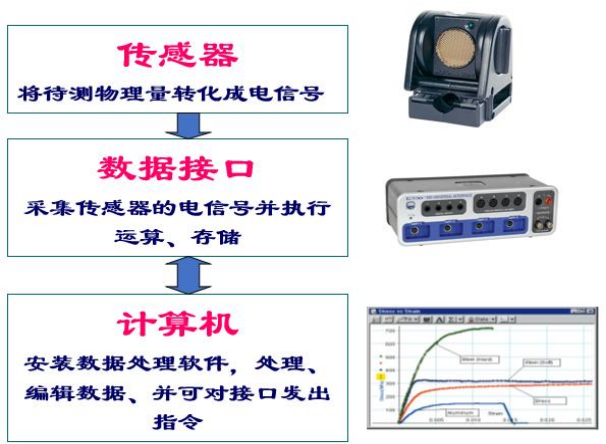
\includegraphics[width=0.6\textwidth]{./fig/计算机实测流程图.png}
  \caption{计算机实测流程}
  \label{fig:计算机实测流程}
\end{figure}
从图\ref{fig:计算机实测流程}
可见。需要传感器将待测信号转换为电信号, 传感器的工作原理是将非电信号转换为电信号, 传感器的输出信号是电信号, 传感器的输入信号是非电信号。之后通过数据接口采集数据,利用计算机进行数据处理,最后进行数据分析和实验报告。
\subsubsection{ RL 串联电路测电感}
使用 RL 电路测量电感, 如图\ref{fig:RL串联电路测电感}所示
\begin{figure}[H]
  \centering
  % \includegraphics[width=0.6\textwidth]{../fig/RL串联电路测电感.png}
  \begin{circuitikz}
    \draw (0,0) to[sV,l=$U_0$] (0,3)
                to [R=$R$] (5,3)
                to [L=$L$,a=$R_L$] (5,0)
                to [short,a=$I$] (0,0);
    \draw (1,3) to [short,*-] (1,4.5) 
                to [rmeter, t=V, straight instruments,l=$U_R$] (4,4.5) 
                to [short,-*] (4,3);
    \end{circuitikz}
    \caption{RL 串联电路测电感电路图}
    \label{fig:RL串联电路测电感}
\end{figure}
如图\ref{fig:RL串联电路测电感}
所示, 电源 $U_0$ 串联电阻 $R$ 和电感 $L$, 电流 $I$ 通过电路, 电感两端电压 $U_L$ 与电阻两端电压 $U_R$ 之比为
\begin{equation}
  \frac{U_L}{U_R} = \frac{R_L}{R}
\end{equation}
其中 $R_L$ 为电感的感抗
\begin{equation}
  R_L = \omega L
\end{equation}
式中 $\omega = 2\pi f$ 为角频率, $f$ 为频率, $L$ 为电感, 电感的感抗 $R_L$ 与电阻 $R$ 之比为
可以求得电路阻抗:
\begin{align}
  &X_L=2\pi fL=\omega L \\
  &R=R_L+R_0\\
  &Z^2=R^2+X_L^2=(R+R_0)^2+(\omega L)^2
\end{align}
用 $R_0$ 写电路电流:
\begin{equation}
  I=\frac{U_R}{R_0}
\end{equation}
阻抗写成:
\begin{equation}
  Z=\frac{U_0}{I}=\frac{U_0}{U_R}R_0
\end{equation}
可以得到
\begin{equation}
  (R+R_0)^2+(\omega L)^2=(\frac{U_0}{U_R}R_0)^2
\end{equation}
可见通过改变频率 $f$ 测量 $U_R$ 再做出 $Z^2-\omega^2$ 进行线性拟合 $Z^2-\omega^2=a\omega^2+b$,可以求得电感的大小 $L$ (即斜率开平方)。
\subsection{实验仪器}
实验使用传感器和计算机软件 PASCO Capstone 进行数据采集和处理、PASCO 550数据接口、电压传感器CI-6503。使用的 PASCO 550数据处理软件PASCO Capstone 及匝数为 400 匝的待测电感。

% \longLine  
\section{实验内容及具体步骤}
\begin{enumerate}
  \item 打开 PASCO 550 数据接口,并通过导线及电压传感器 CI-6503 连成 RL 串联电路。
  \item 打开数据处理软件 PASCO Capstone,如图 7 所示,将硬件设置中通道 A 改成电压传感器,并将信号源输出处选择输出电压传感器。
  \item 将数据的采样频率调至 10KHz,并将交流电的频率依次设置为 100Hz、300Hz、500Hz、600Hz、700Hz 进行采样。
  \item 开始采样后,待有数据采样成功后,迅速停止采样,并用正弦函数对采样出的图像进行拟合。
  \item 表格中记录每个频率的交流电下,拟合后的正弦函数的峰值 A(即为 $R_0$ 两端电压 $U_R$ )。再通过各组数据画出 $Z^2-\omega^2$ 图像,并通过斜率求出电感的感抗值。
\end{enumerate}

\longLine  
\section{数据记录及数据处理}
\subsection{实验数据记录}
获得实验数据如下
\begin{table}[H]
  \centering
  \caption{实验数据记录}
  \label{tab:实验数据记录}
  \begin{tabular}{lllll}\hline
  f(Hz) & $\omega$    & $U_{R_0}(V)$  & $U_0(V)$ & $R_0(\Omega)$  \\ \hline
  100   & 628  & 4.87 & 5  & 100 \\
  200   & 1260 & 4.86 & 5  & 100 \\
  300   & 1880 & 4.85 & 5  & 100 \\
  500   & 3140 & 4.83 & 5  & 100 \\
  700   & 4400 & 4.79 & 5  & 100 \\
  900   & 5650 & 4.74 & 5  & 100 \\\hline
  \end{tabular}
\end{table}
\subsection{数据处理}
进行实验数据处理,计算 $Z^2,\omega^2$ 如表\ref{tab:Z^2-omega^2}所示

使用表\ref{tab:Z^2-omega^2}的数据绘制图像,并进行线性拟合,得到如图\ref{fig:Z^2-omega^2}所示的拟合图像。
\begin{table}[H]
  \begin{minipage}{0.5\linewidth}
  \centering
  \caption{$Z^2-\omega^2$ 数据}
  \label{tab:Z^2-omega^2}
  \begin{tabular}{lll}
    \hline
    f(Hz) & $\omega$       & $Z^2$        \\ \hline
    100   & 394384   & 10541.01 \\
    200   & 1587600  & 10584.43 \\
    300   & 3534400  & 10628.12 \\
    500   & 9859600  & 10716.32 \\
    700   & 19360000 & 10896.05 \\
    900   & 31922500 & 11127.13 \\ \hline
    \end{tabular}
  \end{minipage}
  \begin{minipage}{0.48\linewidth}
    \begin{figure}[H]
      \centering
      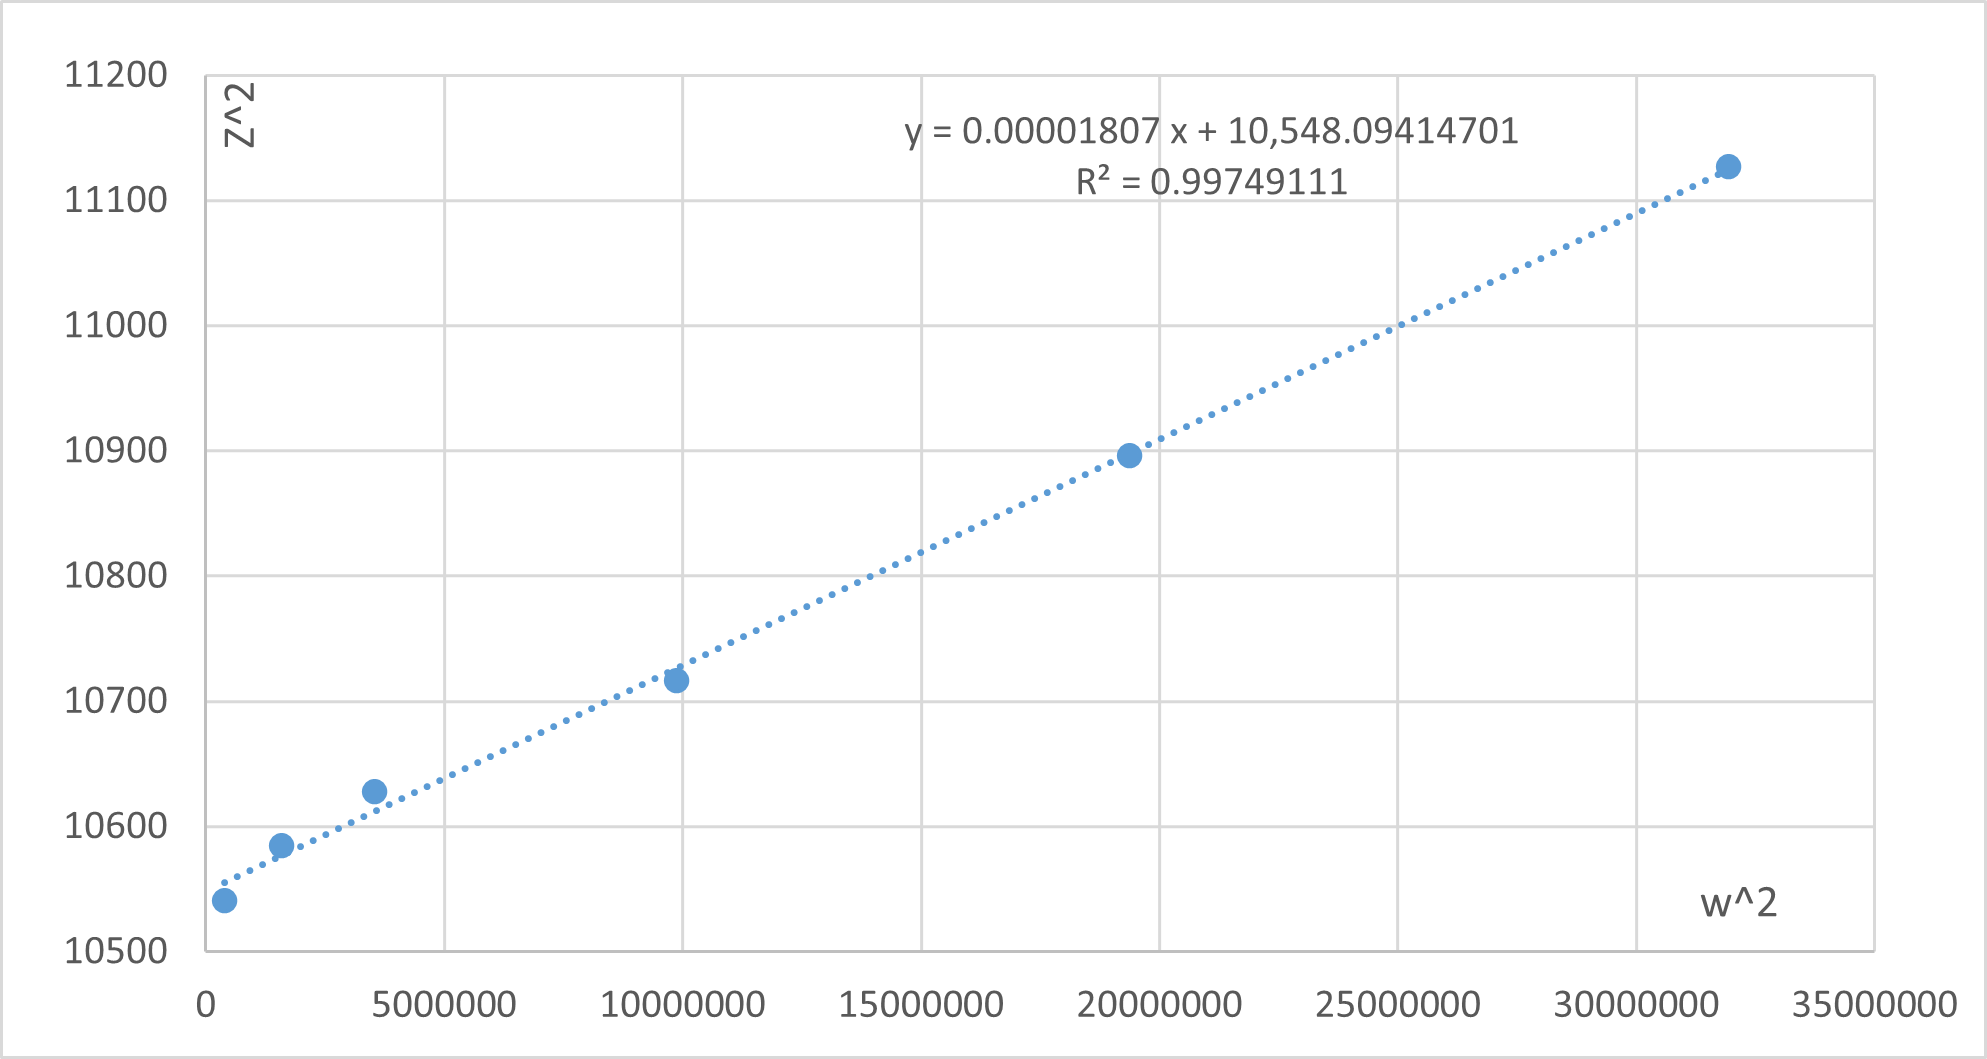
\includegraphics[width=0.95\columnwidth]{./fig/Z^2-omega^2.png}
      \caption{$Z^2-\omega^2$ 数据拟合}
      \label{fig:Z^2-omega^2}
    \end{figure}
  \end{minipage}
\end{table}

如图拟合结果为 $y = 0.00001807 x + 10,548.09414701$,拟合 $R² = 0.99749111$,可见拟合效果较好。

由斜率可得 $L^2 = 0.00001807$,故电感的感抗为:$L=\sqrt{0.00001807}=0.00425H$。由前台仪器测量实际得到电感的感抗为 $2.64mH$,误差为$|\frac{2.64-4.25}{4.25}\times 100\%| = 39.29\%$

\longLine  
\section{实验结果陈述与总结}
\subsection{结果陈述}
通过实验测量多组数据,通过线性拟合得到$y = 0.00001807 x + 10,548.09414701,R² = 0.99749111$电感的感抗为 $4.25mH$,与前台仪器测量的 $2.64mH$ 相比,误差为 $39.29\%$。分析可能是由于电感的内阻等因素导致的误差。
\subsection{实验总结}
通过实验学习了使用 RL 串联测量电感的方法,掌握了电感的测量技术,了解了电感的特性。通过线性拟合求取电感感抗的大小,学习了使用实验数据处理软件 PASCO Capstone 进行数据处理,了解了传感器的工作原理,掌握了传感器的使用方法,这对以后使用计算机辅助物理实验进行数据采集和处理有很大帮助。误差向老师老师助教请教后认为可能与仪器有关,下次实验应该注意仪器的选择使用。

\endBox
\end{document}